\section{Design}\label{sec:design}

\begin{itemize}
	\item Take workflows written in an existing workflow language. Compile
	that into a platform-agnostic abstraction -- unum IR.

	\item The IR represents a workflow as a collection of functions and
	continuations.

	\item Can deploy this IR on any environment that has a serverless system
	and named storage (e.g., blob storage, database, kv store).

	\item There is no separate service executing the workflow. unum functions
	entirely as a library on each serverless function.

	\item Orchestration actions are distributed to component functions in the
	form of continuations during the compilation stage.

\end{itemize}



\subsection{System Requirements}

\begin{itemize}
	\item Any environment that has a serverless offering and a named storage
	\item Named storage = a data store whose items can be accessed by their
	unique names. Examples: object store, database, KV store.
	\item Storage is shared among all functions in a workflow.
	\item Examples: AWS Lambda + s3 or DynamoDB or elasticache
\end{itemize} 



\subsection{Programming Interface and Frontend Compiler}

\begin{itemize}
	\item \name{} does not propose a new workflow programming language
	\item Take workflow written in existing workflow language and transform
	that into a continuation-based IR
	\item Support different types of workflow languages:

		\begin{enumerate}
			\item State machine: AWS Step Functions
			\item DAG: Google Cloud Composer (which is Apache Airflow)
			\item Procedural code DSL: mu/excamera or PyWren (both are limited and
			much less general than Durable Functions) or gg (gg has its own suite
			of applications)
		\end{enumerate}

	\item Give examples on how we tranform. Formal specificiation beyond this paper.
	\item It would be great if we can state a set of necessary characteristics
	of the frontend language that can be compiled into \name{} IR.
\end{itemize}

\begin{figure}[t!]
    \centering
    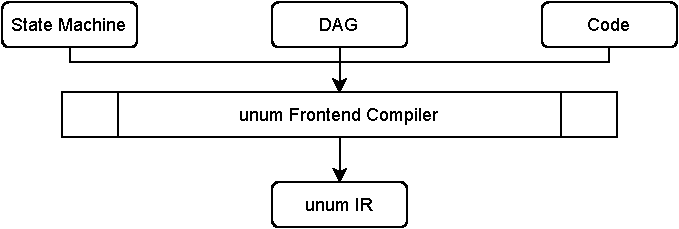
\includegraphics[width=\columnwidth]{figures/unum-frontends.pdf}
\end{figure}

\subsection{\name{} IR}

\begin{itemize}
	\item Represents workflow as serverless functions and continuations.
	\item Continuations are serverless function invocations + input definition.
	\item Each function has 0, 1 or more continuations.
	\item IR extensibility
\end{itemize}
 


\subsection{Runtime}

\begin{itemize}
	\item Runtime is entirely a library running on each serverless function. There
	is no separate server running a specialize coordinator process that
	executes the workflow.
	\item Execute the continuation.
	\item Assigns each invocation a unique name.
	\item Function invocation naming scheme.
\end{itemize}



\subsection{Execution guarantee and fault tolerance}

\begin{itemize}
	\item Exactly-once? At-least-once?
	\item What happens when one of the functions in a large workflow fails? The whole
workflow restart from the beginning? Only the failed function gets retried?
	\item Functions idempotency
	\item \name{} checkpoint knob
\end{itemize}

\subsection{Example Applications}

Walkthrough a few example applications to demonstrate how \name{} expresses and executes at least the following orchestration patterns:
\begin{itemize}
	\item fan-out
	\item fan-in
	\item fold
	\item parallel pipelines
\end{itemize}

Candidate applications (actually we can just describe excamera because it has most of the patterns):

\begin{itemize}
	\item Excamera (patterns: 1. fan-out elements in an array to multiple
	instances of the same function 2. parallel pipelines  3. fold 4. chaining )
	\item image processing (pattern: fan-out the same data to multiple
	functions)
	\item word count (pattern: fan-out elements in an array to multiple
	instances of the same function)
\end{itemize}